\documentclass[10pt,a4paper]{report}
\usepackage[utf8]{inputenc}
\usepackage{amsmath}
\usepackage{amsfonts}
\usepackage{amssymb}
\usepackage{breqn}
\usepackage{graphicx}
\newcommand{\omegav}{{\boldsymbol \omega}}
\newcommand{\xv}{{\bf x}}
\newcommand{\et}{{\bf e}_\theta}
\newcommand{\alphav}{{\boldsymbol \alpha}}
\newcommand{\chiv}{{\boldsymbol \chi}}
\newcommand{\uv}{{\bf u}}
\begin{document}
\begin{huge}
Simulation of Toroidal Vortex Ring(From Ghoniem's paper\cite{ghoniem})
\end{huge}
\section{Geometry and Initial Vorticity Distribution}

Here we look at a toroidal vortex ring with an initial vorticity distribution modeled by a third order Gaussian function:
\begin{equation}
\omegav (\xv) = \frac{1}{a\sigma^2} exp\left(-r_\xv^3/\sigma^3\right) \et
\end{equation} 
\begin{figure}
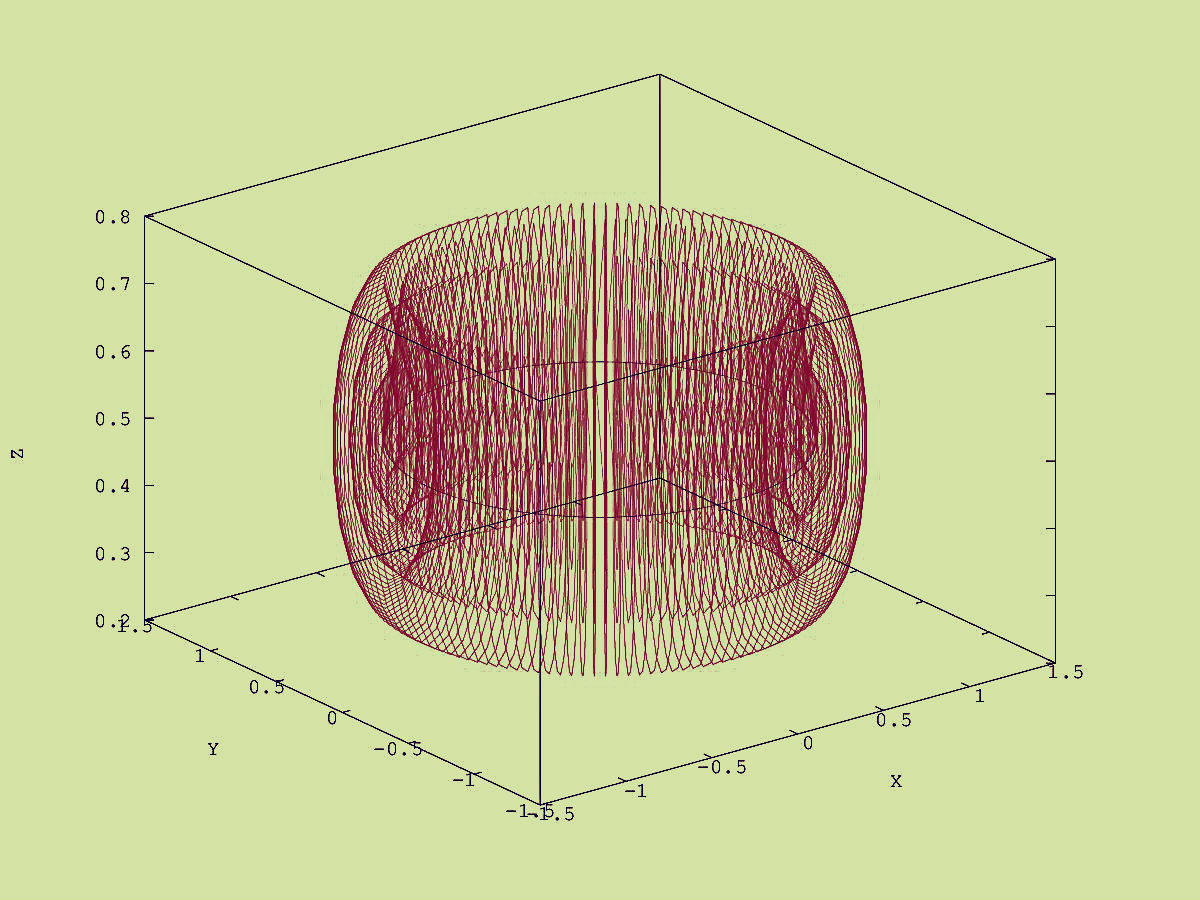
\includegraphics[scale=0.3]{geometry.jpg}
\caption{Vortex Torus with ring axis in blue}
\end{figure}
The vorticity is along the direction $\et$ which is tangential to the ring axis(shown in the figure). The ring axis is the circle, $x^2 + y^2 = R^2$ on the plane $z=z_i$.
The magnitude of the total vorticity is independent of $\theta$ where $(\rho,\theta, z)$ represent coordinates in the cylindrical coordinate system.
\paragraph{}
The cross section of the ring, which is circular, has a radius, $\sigma = 0.275 R$. In the figure, $R = 1$ and $z_i = 0.5$.
\paragraph{}
In a particular cross section,
\begin{itemize}
\item
$r$ is the radial distance measured from the centre of the core of the ring or the centre of a cross section. For all $\xv$ within the ring, $0 \leq r_\xv \leq \sigma $ . 
\item
$\phi$ is the angle measured, at every cross section, from the line passing through the centre of the cross section and parallel to the z axis.  
\end{itemize}
\begin{figure}
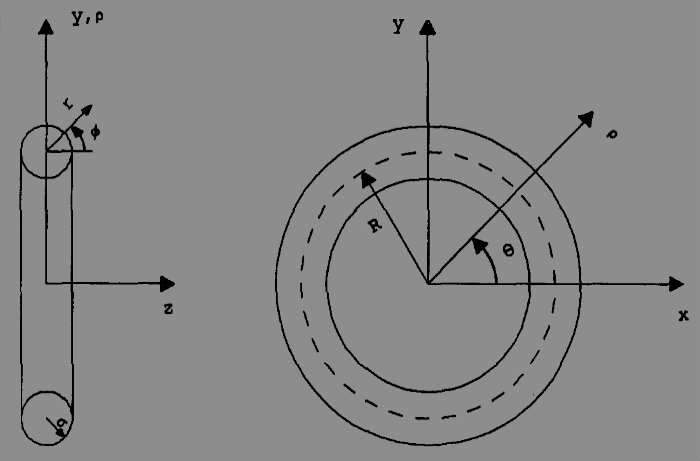
\includegraphics[scale=0.3]{axis.jpg}
\caption{From \cite{ghoniem}}
\end{figure}

\section{Discretization of the Ring}

The toroidal ring is divided into many small vortex tubes. Here, we make an equi-spaced mesh found in the third position on the third row of Fig.11 b of the paper\cite{ghoniem}. The ring is discretized at $N_c$ cross sections and each cross-section is discretized at $N\_per\_ \theta$ locations in total.

Of these $N\_per\_ \theta$ locations, $N_\theta $ points are at each radial location and there are $N_r $ radial locations per cross section. 

In the code, $N_r = 3$ and $N_\theta $ is a multiple of 6. Hence, there are $ N\_per\_\theta = 1 + 6 + 12 + 18 = 37$ elements (including one at the centre) in total per cross section. 

Therefore, the ring is divided into $N = N_c \times N\_per\_\theta $ vortex tubes in total. In the code, $N_c = 120$. Hence, we have $4440$ vortex elements which are part of $N\_per\_\theta $ different vortex tubes.

\begin{figure}
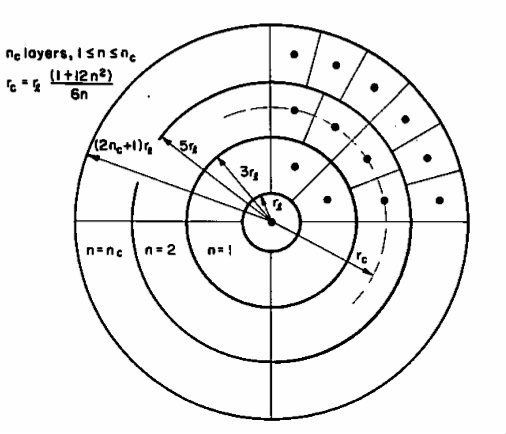
\includegraphics[scale=0.4]{discrete.jpg}
\caption{From \cite{wincklemans} }
\end{figure}

\section{Evaluating Strength Vectors}
In a regularized particle vortex method, the total vorticity field at a given $\xv$ at time t is written as:
\begin{equation}
\omegav(\xv, t) = \sum_{i=1}^N \alphav_i(t) \zeta_\delta( \xv - \xv_i(t)) 
\label{pv}
\end{equation}
where, $ \alphav_i $ is the strength vector associated with the vortex element $i$ whose center is at $ \xv_i $.
And, the regularized core function,
\begin{equation}
\zeta_\delta (\xv - \xv_i) = \frac{1}{\delta^3} \zeta(|\xv - \xv_i|/\delta)
\end{equation}
where
\begin{equation}
\zeta(s) = \frac{15}{8 \pi} \frac{1}{\left(1 + s^2\right)^{7/2}} 
\end{equation}
In the paper\cite{ghoniem}, a Gaussian core function is used. With the above mentioned core function that provides higher order algebraic smoothing\cite{wincklemans}, the accuracy in the total circulation is maintained as well, justifying its selection. 

The Strength Vector, $ \alphav_i $ is actually the contribution to the vorticity of the small vortex tube element $i$ or the product of the element's circulation and length. That is,
\begin{equation}
\alphav_i (t) = \omegav_i dV_i = \Gamma_i \delta \chiv_i
\end{equation} 
Here, $\delta \chiv_i $ is a small length along the vorticity vector (or along a material line). It can be thought of the length of the small vortex tube elements in the Lagrangian system. Therefore, the initial vorticity field, as in Eq:\ref{pv} can be expressed as :
\begin{align}
\omegav(\xv, 0) &= \sum_{i=1}^N \Gamma_i \delta \xv_i \; \zeta_\delta( \xv - \xv_i) \\
				&= \frac{1}{a\sigma^2} exp\left(-r_\xv^3/\sigma^3\right) \et
\end{align}
where, $ \delta \xv_i = \delta \chiv_i(T = 0) $.

The above equations are expressed as a system of linear equations for $\xv$ being each of the $\xv_i$ s or the centres of the elements. Hence, the system of equations solved for the circulation in the $N\_per\_\theta$ vortex tubes can be written as:
\begin{dmath}
\begin{bmatrix}
\displaystyle \sum_{j=1}^{N_c} \zeta_\delta( \xv_1 - \xv_j) \delta \xv_j & \displaystyle \sum_{j=N_c + 1}^{2\times N_c} \zeta_\delta( \xv_1 - \xv_j) \delta \xv_j & . & . &  \displaystyle \sum_{j= N - N_r + 1}^{N_c*N_r} \zeta_\delta( \xv_1 - \xv_j) \delta \xv_j \\ 
\displaystyle \sum_{j=1}^{N_c} \zeta_\delta( \xv_2 - \xv_j) \delta \xv_j & \displaystyle \sum_{j=N_c + 1}^{2\times N_c} \zeta_\delta( \xv_2 - \xv_j) \delta \xv_j & . & . &  \displaystyle \sum_{j=N - N_r + 1}^{N} \zeta_\delta( \xv_2 - \xv_j) \delta \xv_j \\ 
. & . & . & . & . \\ 
. & . & . & . & . \\
\displaystyle \sum_{j=1}^{N_c} \zeta_\delta( \xv_N - \xv_j) \delta \xv_j & \displaystyle \sum_{j=N_c + 1}^{2\times N_c} \zeta_\delta( \xv_N - \xv_j) \delta \xv_j & . & . &  \displaystyle \sum_{j=N - N_r + 1}^N \zeta_\delta( \xv_N - \xv_j) \delta \xv_j \\ 
\end{bmatrix}
 = 
\begin{bmatrix}
\Gamma_1 \\
\Gamma_2 \\
. \\
. \\
\Gamma_N
\end{bmatrix}
\begin{bmatrix}
\frac{1}{a\sigma^2} exp\left(-r_{\xv_1}^3/\sigma^3\right) \\
\frac{1}{a\sigma^2} exp\left(-r_{\xv_2}^3/\sigma^3\right) \\ \\
. \\
. \\
\frac{1}{a\sigma^2} exp\left(-r_{\xv_N}^3/\sigma^3\right) \\
\end{bmatrix}
\end{dmath}

These $N_r$ equations are solved to the give the circulations of the $N_r$ vortex tubes.
It must be noted that $\delta \xv_i $ or the initial length of the vortex tube $i$ depends both on the radial and azimuthal positions of the tube within a cross section or $r$ and $\phi$ respectively.
\begin{equation}
\delta \xv_i = 2 \pi \times ( R + r_{\xv_i} \cos \phi ) 
\end{equation}
($ \xv_i $ is the centre of the $i$th vortex element ).

For the discretization described above, the total circulation of the ring is close to the theoretical value of $2$.
\begin{equation}
\sum_{i=1}^{N_r} \Gamma_i = 2.0546 
\end{equation}

\section{Evolution of Ring}
For the first iteration, with 4400 particles (or vortex elements), direct evaluation and FMM computation were performed for the velocity and the stretching term of each particle.
\begin{align}
\frac{d\xv_i}{dt} &= \uv(\xv_i(t),t) \\
				&=  \frac{-1}{4\pi} \displaystyle \sum_{j=1}^{N} \frac{(\xv_i - \xv_j)^2 + 5/2 \delta^2}{((\xv_i - \xv_j)^2 + \delta^2)^{5/2}} (\xv_i - \xv_j) \times \alpha_j
\end{align}

\begin{align}
\frac{d\delta\chiv_i}{dt} &= \delta\chiv_i . \nabla \uv(\xv_i(t),t) \\
				&=  \frac{1}{4\pi} \displaystyle \sum_{j=1}^{N} \Bigg( \frac{|\xv_i - \xv_j|^2 + 5/2 \delta^2}{(|\xv_i - \xv_j|^2 + \delta^2)^{5/2}} \delta\chiv_i \times \delta\chiv_j \\
				&+ 3 \frac{(|\xv_i - \xv_j|^2 + 7/2 \delta^2)}{(|\xv_i - \xv_j|^2 + \delta^2)^{7/2}} \times \\
				&(\delta\chiv_i.((\xv_i - \xv_j)\times \delta\chiv_j)(\xv_i - \xv_j) \Bigg)
\end{align}

The FMM was accurate upto the 5th decimal place when compared to the direct evaluation. 

 







\begin{thebibliography}{3}
\bibitem{ghoniem} 
\emph{Omar M. Knio and Ahmed F. Ghoniem},Numerical Study of a Three Dimensional Vortex Method,
Journal of Computational Physics,1990

\bibitem{wincklemans}
\emph{G.S. Wincklemans and A. Leonard}
,Contributions to Vortex Particle Methods for the Computation of Three-Dimensional Incompressible Flows,
Journal of Computational Physics, 1993.

\end{thebibliography}

 



 
\end{document}